%% ID: road_collision
%% TITLE: Road Collision
%% TYPE: question
%% QUESTIONTYPE: numeric
%% CONCEPTS:  energy, friction, momentum, NewtonII, zero_momentum_frame, vectors1, vectors2
%% VIDEOS: 
%% LEVEL: 6
%% TOPIC: mechanics/dynamics
%% ORDER: 3

%\input{../../../Templates/Problem_Template}
%\begin{document}
\begin{problem}[Road Collision] %A2-1
{A car of mass 1500 kg was travelling down a motorway when a larger car of mass 2500kg moved in from another lane at an angle of \valuedef{\alpha}{15}{$^{\circ}$} to the direction of the road and collided with it. After the collision these two cars stuck to each other, moving at an angle \valuedef{\theta}{8}{$^{\circ}$} to the direction of the road. They came to a stop 46m from the point of collision. Assuming that the the coefficient of friction between the road and the combined two cars after the collision is 0.7 and no air resistance, find the speeds of the  cars just before the collision.
}
{\textit{Created by MC for the Rutherford Schools Physics Project}}
{Taking \vari{m_1} as the mass of the larger car and \vari{m_2} as the mass of the smaller car, after the collision, the combined cars have a velocity \vari{v}, and hence a kinetic energy $\half (m_1+m_2) v^2$. When they are at rest, all of this kinetic energy has been lost. This loss in KE is equal to the work done by the friction of the road on the cars, given by $W = Fx$.
\begin{equation} \mu (m_1+m_2)gx = \half (m_1+m_2) v^2 \end{equation}
\begin{equation} v = \sqrt{2\mu gx} \end{equation}

\begin{figure}[h]
\centering
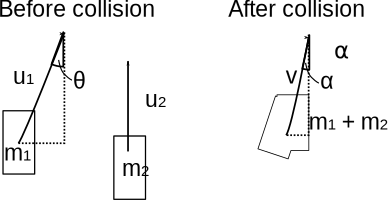
\includegraphics[scale =1]{dynamics_l6_car_collision}
\caption{}
\label{fig:dynamics_l6_car_collision}
\end{figure}


By conservation of momentum in the direction at ninety degrees to the main road 
\begin{equation} m_1 u_1  \sin \alpha = (m_1+m_2)v  \sin \theta  \end{equation}
\begin{equation} u_1 =  \frac{(m_1+m_2) \sqrt{2\mu gx}\sin \theta}{m_1 \sin \alpha}\end{equation}
giving \valuedef{u_{1}}{21.5}{m\,s$^{-1}$}.
Similarly, by conservation of momentum along the motorway 
\begin{equation} m_1 u_1 \cos \alpha + m_ 2 u_2 = (m_1+m_2) v \cos \theta \end{equation}
\begin{equation} u_2 =   \frac{(m_1+m_2) \sqrt{2\mu gx}\cos \theta - m_1 u_1  \cos \alpha}{m_2}\end{equation} \valuedef{u_2}{31.7}{m\,s$^{-1}$}
}
\end{problem}
%\end{document}


